%% The report will be no longer than 3 pages and will include the following:
% 1. Verification of the generality of your A* algorithm. Any aspect of A* that 
% is specifically geared toward CSP and GAC should be in subclasses, not the 
% core A* classes.
% 2. Verification of the generality of your A*-GAC algorithm. Any aspect of 
% A*-GAC that is specifically geared toward VC should be in subclasses, not the 
% core code. You will be reusing A*-GAC on other assignments, so the core should
% be easily extendable via subclassing.
% 3. Verification of a clean separation between your Constraint Network (CNET) 
% and the VIs and CIs of the search states, as shown in Figure 4.
% 4. A clear explanation (with small code segments) of: a) the manner in which 
% your system creates code chunks on the fly, or b) the general workings of your 
% hand-built interpreter for executing constraints in a canonical form, or c) 
% your work-around for avoiding both code chunks and a hand-built interpreter.

\section{Central aspects of your A*-GAC program}
This report describes our implementation of the A*-GAC and our solution to the vertex coloring problem.

\subsection{Generality of the A* and the A*-GAC}
Two classes must be subclassed to solve new problems; the BestFirstSearch class and the SearchState class. To utilize the power of the GAC, it has to be run on every generated node, even the root node. So in the subclass of BestFirstSearch, the `create\_root\_node' method must be overidden to perform both gac.initialize() and gac.domain\_filtering(), as seen in code snippet \ref{code:create_root}.

\lstinputlisting[emph={create_root},label={code:create_root},caption={Generation of root node.}]{module_2/code_snippets/create_root.py}

Further, the GAC has to be rerun on each generated successor in the overidden method `generate\_all\_successors', before it gets added to the open heap. Only successors which either got solved by the GAC, or did not get one or more of their domains reduced to an empty domain \( D = \{ \emptyset \}\), is considered as a valid child and should be expanded. The `gac.rerun()' returns \(True\) if the successor is still a viable state after the GAC-reduction. If the state is viable, it gets added to the opened heap in the A* agenda.

\lstinputlisting[emph={GAC},label={code:successor_generation},caption={Generation of vertex successor states.}]{module_2/code_snippets/successor_generation.py}

The A*-GAC-program uses directly the generalized GAC class we have written, that contain the initialize, domain\_filtering and rerun methods. However, when a graph is read and we create the constrains, we do so with a specialized VertexConstraint class which inherits a generalized Constraint class. The generalized constraint class implements the revise algorithm. The specialized VertexConstraint can parse the type of expressions used by the VertexColoring search, and implements a method for reversing an expression. The constraints we have used in module 2 are of the form 'vx != vy'. VertexColoring contains a method that parses variables from these expressions by excluding '!=', and a method for generating the expression 'vy != vx' as our GAC class uses both forms of the expression. This becomes important in module 3.

\begin{figure}[h!]
  \centering
    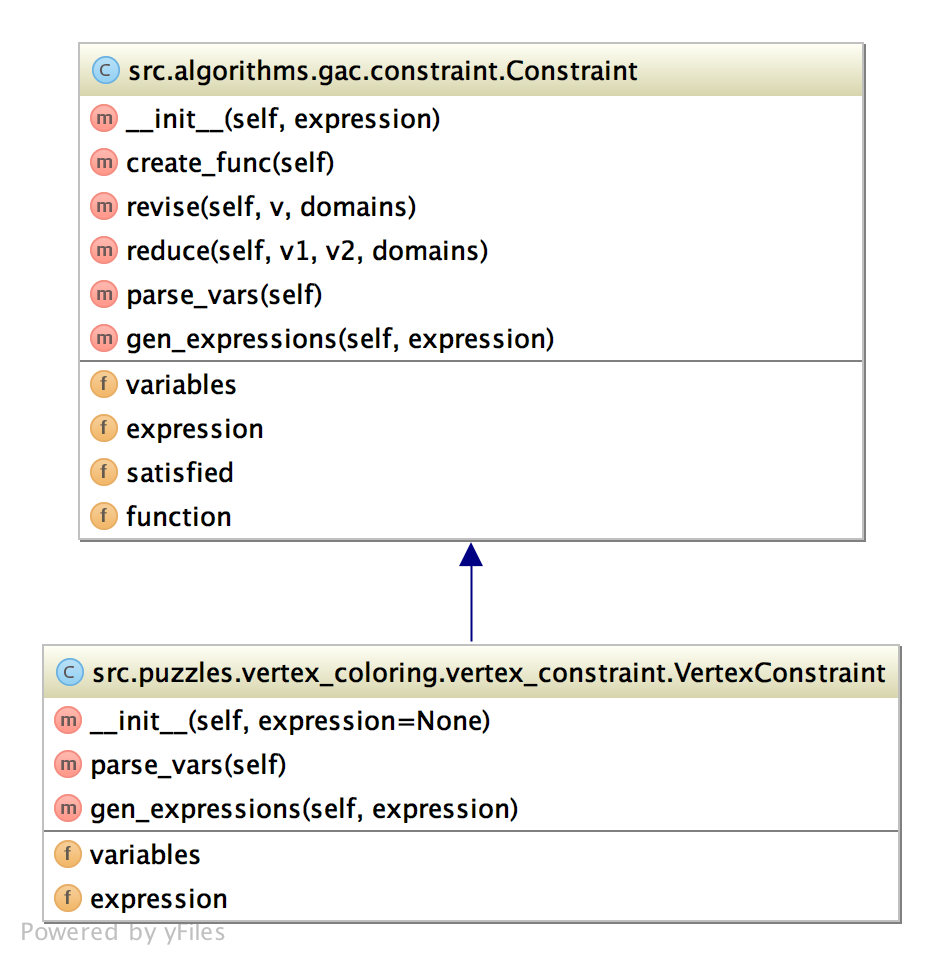
\includegraphics[width=0.5\textwidth]{module_2/images/vertex_constraint}
  \caption{Class diagram for the constraint implementation. }
  \label{constraint:vertex}
\end{figure}

\subsection{CNET, VIs and CIs}
The domains, constraints and variables are only generated once and shared between the different classes. A dictionary in the GAC maps the variables to the constraints, so the constraints can easily be looked up by a variable.

The constraints (CIs) is generated as runnable expressions, as in this problem: \( v1 \neq v3 \), where \(v1\) and \(v2\) represent the vertices. In previous example, vertex \(v1\) and \(v2\) should not have the same color. The variable instances (VIs) is being stored as list of strings in each constraint, as involved variables. These variables are used to retrieve the domains from a dictionary that is initialized at `gac.initialize()'. Each node has its own dictionary with references to variable domains. If a domain is being altered, a copy of this domain is being made and the reference is updated in the corresponding state.

\subsection*{Heuristics}
It's two heuristics at play, one that selects the successors and one that determines which node to get expanded first. For the selection of successors, we simply select the variable that has the smallest domain and create states for all colors in this variables' domain; one assumption for each color.

If the A* has to pop a node from the heap, it looks at the solution domain, which equals the amount of nodes available, and picks the node that result in the smallest solution domain. This means we have cut off the domain of possible combinations of colored graphs. Let's look at an example of computing the size of the solution domain:

\begin{align*}
	&v1: [0,1,2,3]\\
	&v2: [0,2]\\
	&v3: [2,3,4]
\end{align*}

Here we have \(4 \cdot 2 \cdot 3 = 24\) possible combinations of the given colors, some of the states are not viable though, but it is still a good measure and the nonviable states can - with no loss in performance - be neglected. The catch, though, is that while multiplying a lot of these values, you get a heavily incrementing value, and can give a negative boost on the performance of the solver. To solve this, we chose to take the logarithmic value of the length of the domains and add all those together. As most know, adding values in the logarithmic scale, is equal multiplying the original values. So we'll get the correct measurement, but in another representation. Another property of this heuristic is that when all domain lengths equal 1, the heuristics equals 0. Our heuristics function is provided in code snippet \ref{code:heuristics}.

\lstinputlisting[label={code:heuristics},caption={A* Heuristics used for the vertex coloring problem.}]{module_2/code_snippets/heuristics.py}

\subsection{Evaluation procedure of the GAC}
The REVISE method is a regular REVISE, and not a REVISE* as described in the problem description. This is because REVISE* is not necessary to solve the modules provided in the course this year. We chose to focus on optimizing the problem at hand.

\lstinputlisting[label={code:make_function},caption={Generation of lambda expressions to evaluate the constraints.}]{module_2/code_snippets/make_functions.py}

Two functions are produced for each constraint, e.g. \( v1 \neq v2 \) produces both \(v1 \neq v2 \) and \(v2 \neq v1 \). The revise chooses which function to use based on the focus variable given. This avoids expressions that look up values in lists to return falsy values, e.g. \( v1[0] \neq v2[1] \) should not return the result of \( v2[0] \neq v1[1] \). The latter is especially important in the next module. To create runnable functions, we use Python's lambda function, as seen in code snippet \ref{code:make_function}. To run the function you simply do as shown in the code snippet \ref{code:apply_function}. In the code snippet, \(v1\) is the focus variable, \(d1\) is its value and \(d2\) is the other variables' value.

\lstinputlisting[label={code:apply_function},caption={Applying a lambda function.}]{module_2/code_snippets/apply_function.py}